% !TEX encoding = UTF-8
% !TEX TS-program = pdflatex
% !TEX root = ../tesi.tex

%**************************************************************
\chapter{Analisi comparativa dei protocolli REST e GraphQL}
\label{cap:analisi-comparativa}
%**************************************************************
\intro{In questo capitolo verrà svolta l'analisi comparativa tra i due protocolli REST e GraphQL, sia dal punto di vista teorico che da quello pratico .}\\
%**************************************************************
%\section{Analisi comparativa teorica}
%\label{sec:analisi-comparativa-teorica}
%Per analisi comparativa teoria s'intende tutti quegli aspetti che differenziano i due protocolli GraphQL e REST
\section{Introduzione}
REST è stato ed è tutt'oggi lo standard più seguito per la realizzazione delle Web API, tuttavia dopo l'uscita di GraphQL gli sviluppatori hanno iniziato ad utilizzare sempre di più la nuova tecnologia. Infatti GraphQL ha portato con se delle interessanti soluzioni per molti dei problemi e dei vincoli dello stile architetturale REST.\\
L'innovazione portata da GraphQL è stata apprezzata in larga scala tra gli sviluppatori, a conferma di ciò è possibile visualizzare nell'immagine \ref{graphQL-usage-chart} l'aumento nell'utilizzo di questa tecnologia con il passare degli anni.
\FloatBarrier
\begin{figure}[!ht]
\centering
\includegraphics[width=1\linewidth]{immagini/GraphQLUsageChart.png}
\caption{Grafico sull'utilizzo di GraphQL negli anni.}
\label{graphQL-usage-chart}
\end{figure}
\FloatBarrier
Nel seguente capitolo verranno analizzati nel dettaglio e paragonati i due protocolli, sotto tutti i punti di vista, mettendo in risalto vantaggi e svantaggi di ciascuno; infine verranno riportate le deduzioni elaborate durante lo stage sul protocollo che è meglio seguire in base all'applicativo che si vuole sviluppare.
\section{Analisi comparativa}
Come sottolineato in precedenza, GraphQL e REST hanno diversi aspetti che li differenziano. La più grande differenza tra questi due protocolli è legata alla loro natura: infatti quando si fa riferimento a REST, si sta parlando di uno stile architetturale, dunque di un modo di costruire le proprie API le quali, se rispettano i vincoli REST illustrati al punto \ref{principi-REST}, vengono definite RESTful. Quando si fa riferimento a GraphQL invece, si sta parlando di un linguaggio di query fortemente tipizzato.\\\\
Di seguito è presente un'analisi comparativa dettagliata per ciascun aspetto che differenzia i due protocolli di data fetching.
\subsection{Endpoints}
La prima grossa differenza tra i due protocolli riguarda gli endpoint.\\
Lo stile REST prevede l'utilizzo di più endpoint, sfrutta infatti la molteplicità degli endpoint per differenziare le richieste possibili. Quando un client implementa una richiesta a delle REST API deve sapere esattamente a quale endpoint inviare la richiesta per ricevere i dati necessari. In figura \ref{REST-endpoints} viene rappresentato la struttura degli endpoint multipli di un REST server con il client che invia diverse richieste ai diversi endpoint.
\FloatBarrier
\begin{figure}[!ht]
\centering
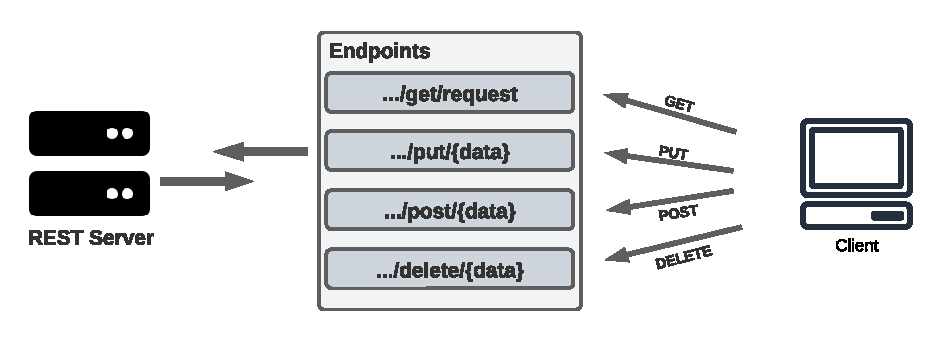
\includegraphics[width=1\linewidth]{immagini/RESTEndpoints.pdf}
\caption{Gli endpoints multipli in REST.}
\label{REST-endpoints}
\end{figure}
\FloatBarrier
Con GraphQL questo non avviene, infatti GraphQL prevede l'esposizione di un unico endpoint. A questo singolo endpoint possono essere inviate tutte le richieste inserendo nel body della richiesta la query, la mutation o la subscription. In figura \ref{GraphQL-endpoint} è possibile visualizzare come il GraphQL server fornisca un unico endpoint e come il client invii tutti i tipi di richieste allo stesso medesimo endpoint.
\FloatBarrier
\begin{figure}[!ht]
\centering
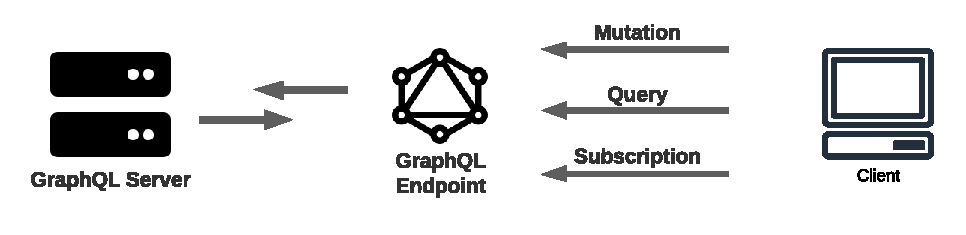
\includegraphics[width=1\linewidth]{immagini/GraphQLEndpoint.pdf}
\caption{Il singolo endpoint GraphQL.}
\label{GraphQL-endpoint}
\end{figure}
\FloatBarrier
A proposito di ciò viene riportata di seguito una citazione di Lee Byron, il co-creatore di GraphQL:
\begin{quoting}
  \textit{"Think in graphs, not endpoints."}
\end{quoting}
\subsection{Overfetching e Underfetching}
La questione dell'overfetching e underfetching è uno degli aspetti che viene maggiormente considerato nella decisione architetturale riguardo quale protocollo di data fetching utilizzare tra REST e GraphQL.\\
Lo stile architetturale REST non prevede di definire lato client esattamente quali dati ricevere. Un client che necessita un certo insieme da un server con REST API, è costretto ad eseguire una o più richieste e dunque a prendersi in carico della rielaborazione dei dati. Per uno sviluppatore backend è molto complesso riuscire a creare delle REST API che siano in grado di soddisfare esattamente le tutte le richieste dei client.
L'introduzione di GraphQL come nuovo protocollo di data fetching ha posto una soluzione a questo problema, permettendo al client di specificare esattamente la forma e il quantitativo di dati necessari. Quando si decide di implementare un applicativo e si valuta quale protocollo di data fetching utilizzare, questo è sicuramente un punto da considerare.\\
\paragraph{Overfetching}
Quando si parla di overfetching si fa riferimento al fatto che vengano forniti più dati di quanti realmente necessari. Riprendendo come esempio il prototipo visto nel capitolo \ref{casi-uso}, si suppone che il client necessiti della lista degli impiegati e che, per ciascun impiegato, necessiti  esclusivamente l'id e il nome. Qualora si tratti della version REST del server, il client inviare la richiesta HTTP all'endpoint mappato sul metodo \textit{allEmployee()}, il quale ritorna una lista di impiegati e, per ciascun impiegato, tutti i campi. Di seguito il JSON di risposta che il client riceve in seguito alla richiesta nel caso in cui fossero presenti solo due impiegati:
\begin{verbatim}
  [
    {
        "id": "3AFASDF12F",
        "name": "Matteo",
        "surname": "Verdi",
        "salary": 1500,
        "birth": "1995-02-21"
    },
    {
        "id": "GA14PL3FAV",
        "name": "Marco",
        "surname": "Blu",
        "salary": 1500,
        "birth": "1993-12-20"
    }
  ]
\end{verbatim}
Si può subito notare come i campi \textit{surname}, \textit{salary} e \textit{birth} non siano necessari in quanto il client utilizza solo i campi \textit{id} e \textit{name}. Nel caso del prototipo si tratta di un problema irrisorio data la ridotta grandezza dei dati, tuttavia in applicativi a larga scala che richiedono grossi quantitativi di dati complessi può risultare un problema in termini di occupazione di rete e di rallentamenti dell'applicativo. Questo problema può essere risolto in un server con REST API fornendo endpoint specifici per ciascun tipo di richiesta, tuttavia questa soluzione rischia di introdurre confusione e nel tempo la manutenzione potrebbe risultare sempre più complessa.\\
GraphQL risolve questo problema attribuendo al client la responsabilità di definire quali siano i campi di cui necessita. Questo è possibile specificando nella query i campi richiesti, di seguito l'esempio dell'invocazione contenente a sinistra la query \textit{allEmployees}, mentre a destra il JSON ricevuto in risposta:
\begin{verbatim}
    QUERY                                     JSON RETURNED

    query {                              "data": {
      allEmployees {                        "allEmployees": [
          id                                  {
          name                                   "id": "3AFASDF12F",
          }                                      "name": "Matteo"
        }                                     },
      }                                       {
                                                 "id": "GA14PL3FAV",
                                                 "name": "Marco"
                                              }
                                            ]
                                          }
\end{verbatim}
In GraphQL questo approcio permette di non sovraccaricare inutilmente la rete e di mantenere ordinato e di facile manutenzione la struttura API del server. Lato client è richiesto un maggior sforzo nella specifica della query, ma d'altra parte si evitano problemi di rallentamento o errori dovuti al fetching di grossi quantitativi di dati inutili.
\paragraph{Underfetching}
L'underfetching è il problema opposo all'overfetching, ovvero ciò accade quando il client dopo una richiesta alle REST API riceve solo una parte dei dati necessari. Questo implica che il client deve eseguire più chiamate per ottenere i dati completi.\\
Riprendendo l'esempio precedente nel paragrafo riguardante l'overfetching, qualora il client desiderasse visualizzare i progetti ai quali sta lavorando un impiegato, dovrà prima ricevere la lista degli impiegati e, solo successivamente, ricercare i progetti con l'id dell'impiegato.\\
La stessa medesima operazione utilizzando GraphQL è risolvibile in una sola richiesta:
\begin{verbatim}
  QUERY                                 JSON RETURNED

  query {                           "data": {
    allEmployees {                     "allEmployees": [
      id                                 {
      projects {                           "id": "3AFASDF12F",
          id                               "projects": [
          name                               {
        }                                       "id": "7NFAISH280",
      }                                         "name": "Progetto Beta"
    }                                        },
  }                                          {
                                                "id": "N2A8F234SD",
                                                "name": "Progetto Teta"
                                            }
                                           ]
                                          }
                                        ]
                                      }
\end{verbatim}
A sinistra è possibile visualizzare la query \textit{allEmployees} nella quale viene specificato l'id di ciascun impiegato ed il campo \textit{projects}, il quale, a sua volta, ha specificato i campi \textit{id} e \textit{name}. A destra invece è visualizzato il JSON ritornato con l'impiegato e i due progetti ai quali sta partecipando.
\subsubsection{Utilizzo del protocollo HTTP}
Nonostante entrambi i protocolli non richiedano per forza il protocollo HTTP per funzionare, entrambi nella maggior parte dei casi vengono utilizzati con esso. Per questo motivo viene eseguita un'analisi su come REST e GraphQL si comportano con il protocollo HTTP. \\
I due protocolli comparati utilizzano il protocollo HTTP in maniera molto differente. Lo stile REST alla sua creazione è stato fortemente basato sul protocollo HTTP, per questo motivo lo sfrutta ampiamente. GraphQL invece, per il modo in cui opera, sfrutta solo in parte ed in maniera "stupida" il protocollo HTTP e per questo motivo GraphQL viene spesso definito agnostico rispetto al protocollo di trasporto.
\paragraph{Metodi HTTP}
Per metodi HTTP s'intendono le possibili operazioni che il protocollo HTTP prevede nella comunicazione tra due moduli di rete. Le API REST supportano i metodi POST, GET, PUT e DELETE per la gestione delle risorse sul server e nel caso della POST e della PUT è possibile specificare i dati all'interno del body della richiesta HTTP. GraphQL invece sfrutta solamente l'operazione POST e specifica nel body la query, la mutation o la subscription desiderata.
\paragraph{Codici di stato}
I codici di stato vengono utilizzati per dare informazioni sull'esito di una richiesta HTTP e risultano fondamentali nella comprensione degli errori. Mentre REST utilizza ampiamente i codici di stato nelle risposte, GraphQL ritorna esclusivamente il codice di stato 200 e specifica il problema nel JSON ritornato; talvolta in alcuni GraphQL server, qualora si dovessero verificare degli errori, può essere ritornato anche il codice di stato 500 riferito all'\textit{Internal Server Error}.
\paragraph{Caching}
Per caching s'intende il meccanismo attraverso il quale il browser, il client, i server proxy o altri moduli della rete riescono ad archiviare localmente i dati a cui si accede frequentemente senza dover ogni volta mandare la medesima richiesta al server. Si tratta di fattore importante poiché, se utilizzato correttamente, permette di ridurre il traffico dati tra i moduli della rete e i tempi di latenza, i dati sono recuperabili molto più velocemente e questo è fondamentale per fornire velocemente i dati nei siti web, vengono eseguiti meno accessi al database lato server e le performance di conseguenza migliorano.\\
Il caching è parte integrante del protocollo HTTP e viene ampiamente sfruttato in REST, infatti per il metodo GET e in parte anche per i metodi PUT e DELETE il caching, a meno di direttive specifiche, viene utilizzato di default. Per quanto riguarda il metodo POST il caching non viene utilizzato di default, ma con apposite direttive nell'header della risposta HTTP è possibile permetterlo.\\
Per il modo in cui opera GraphQL, il caching previsto dal protocollo HTTP non viene sfruttato. Per questo motivo, anche nella documentazione GraphQL, viene specificato come sia un dovere del client quello di abilitare e gestire il caching. Alcune librerie permettono di risolvere questo problema, ad esempio il modulo \textit{Apollo} utilizzato per la realizzazione del frontend del prototipo e nella migrazione dell'applicativo SushiLab, include una implementazione del caching di default chiamata \textit{InMemoryCache}.
\subsubsection{Altri aspetti comparativi}
Sono presenti molti altri aspetti che differenziano i due protocolli analizzati. Di seguito vengono riporatati i più importanti.
\paragraph{Documentazione}
La documentazione delle API risulta fondamentale quando uno sviluppatore client necessita di utilizzare i servizi web resi disponibili da un server.\\
Uno degli aspetti più interessanti di GraphQL è proprio quello che si autodocumenta durante la definizione del GraphQL Schema. Infatti definendo il GraphQL schema vengono dichiarati i tipi e la loro struttura campo per campo, le loro relazioni, le query, le mutation, le subscription ed eventuali altri tipi particolari come tipi unione ed enumerazioni. Inoltre il linguaggio SLD, utilizzato nella realizzazione dello schema GraphQL, supporta anche il linguaggio di markup \textit{Markdown} e dunque è possibile, direttamente dal GraphQL schema, specificare ulteriori informazioni su determinati elementi dello schema inserendo delle frasi.\\
Lo sviluppatore client che desidera la documentazione su un determinato schema GraphQL, può facilmente recuperarla con un processo chiamato \texit{Introspection} per il quale è possibile effettuare una query sempre disponibile richiedendo il campo \textit{\_\_schema} e definendo ciò che vuole visualizzare dei tipi nello schema, così facendo può ottenere come risposta direttamente tutte le informazioni che più desidera. Ci sono inoltre dei tool che permettono di semplificare il processo di instrospezione, ad esempio usando il GraphQL playground.\\
In REST non è previsto nessun modo per documentare le API se non affidandosi a servizi esterni, come ad esempio il noto toolset opensource \textit{Swagger}.
\paragraph{Sicurezza}
Si tratta di un fattore fondamentale per la trasmissione sicura di dati tra moduli sulla rete. Le REST API supportano i protocolli crittografici, ad esempio il Transfer Layer Security il quale assicura che i dati che vengono passati tra moduli della rete rimangano invariati e privati. Inoltre sono presenti moltpelici specifiche per garantire la sicurezza nello scambio di messaggi attraverso API REST, tra le quali: JWT, JWS, JWk, ecc...\\
Anche GraphQL ha dei modi per l'autenticazione e l'autorizzazione le richieste del client, tuttavia risultano sicuramente meno sviluppati e consolidate rispetto a quelli disponibili con le REST API.\\
Un altro punto critico di GraphQL legato alla sua flessibilità, ovvero al fatto che permetta di richiedere qualsiasi tipo di dato in qualsiasi forma, è quello che proprio per questa ragione sia possibile, se non vengono strutturate bene le risorse, essere vittime di attacchi DoS attraverso query annidate che vanno a sovraccaricare il database e il server. Questa parziale mancanza di GraphQL è dovuta probabilmente al fatto che si tratti di una tecnologia giovane, ma sono presenti sempre più modi per gestire la sicurezza ed evitare questo tipo di situazioni.
\paragraph{Formato dati supportati}
Le REST API supportano diversi tipi di dati come: JSON, XML e YAML. GraphQL dall'altra parte supporta solo il formato JSON.
\paragraph{Versionamento ed evoluzione delle API}
Il versionamento e l'evoluzione delle API sono argomenti molto dibattuti, ci sono diversi filoni di pensiero e diversi approci classici, alcuni prediligono l'evoluzione delle API, altri ritengono necessario versionarle.\\
GraphQL predilige un approcio di evoluzione delle API, infatti è possibile evolvere le proprie GraphQL API introducendo nuovi campi nei tipi e preservando i vecchi campi così da mantenere la retrocompatibilità. A conferma di quanto appena affermato, di seguito viene riportato quanto scritto nella pagina riguardante le migliori pratiche nella documentazione GraphQL:
\begin{quoting}
  \textit{"While there’s nothing that prevents a GraphQL service from being versioned just like any other REST API, GraphQL takes a strong opinion on avoiding versioning by providing the tools for the continuous evolution of a GraphQL schema."}
\end{quoting}
Questo approcio inoltre può essere utilizzato anche con API REST.\\
Per quanto riguarda però l'eliminazione di alcune funzionalità o campi dati, in GraphQL è possibile definire dei campi deprecati con apposite direttive e, quando gli sviluppatori frontend interrogano lo schema con l'introspezione, vengono scoraggiati dall'utilizzare quella determinata funzionalità o campo dati che verrà presto rimossa. A differenza degli schemi di versionamento come il \textit{Semantic Versioning}, in GraphQL non è possibile specificare quando verrà rimosso effettivamente il campo deprecato. Anche con le REST API può essere indicato un campo deprecato, ma questo è possibile specificarlo solo nella documentazione delle API.\\
Dunque in accordo con quanto riportato precedentemente dalla documentazione GraphQL, nulla impedisce il versionamento in GraphQL, per questo sono stati ideati dei modi per versionare anche le GraphQL API, come ad esempio includere nei vari tipi dei campi versionamento e dunque in base alla versione trattare i vari campi in maniere differenti. In REST invece il versionamento avviene in maniera differente, infatti vengono utilizzati principalmente due approci, uno che prevede di realizzare più versioni di API e richiede però che venga specificato la versione nell'URI della chiamata; l'altro che invece richiede di specificare la versione includendola nell'header della richiesta HTTP.
\paragraph{Trasmissione di dati in tempo reale}
Nelle Real Time Application è necessario ricevere i dati dal server in tempo reale. Questo non è possibile se il server fornisce delle REST API, a meno che non vengano utilizzati degli escamotage come ad esempio il \textit{long pooling} secondo il quale il server, dopo aver ricevuto una richiesta dal client, mantiene aperta la connessione fino a che non arrivano dati in tempo reale e quel punto invia la risposta al client, il quale subito dopo invia una nuova richiesta al server per riaprire immediatamente la connessione.\\
In GraphQL non serve utilizzare degli escamotage per permettere questo tipo di scambio dati in tempo reale, infatti è stato reso disponibile un tipo detto \textit{Subscription}, spiegato precedentemente nel capitolo \ref{casi-uso}, che permette al client di "iscriversi" ad un certo tipo di dati e, al verificarsi di un certo evento, il server invia direttamente i dati al client senza che il client li richieda. Il tutto è implementato con i WebSocket che permettono di mantenere la connessione server-client attraverso una connessione TCP. \\
È possibile utilizzare in WebSocket anche con API REST, ma risulta essere comunque un adattamento guidato da esigenze di poter utilizzare connessioni bidirezionali, non come nel caso di GraphQL in cui si tratta proprio di una funzionalità prevista dal protocollo stesso.
\paragraph{File uploading}
Spesso può essere necessario permettere al client di effettuare l'upload di file di vario genere sul server. In REST questa necessità viene soddisfatta pienamente, infatti è possibile passare il file inserendolo nel body della richiesta e impostanto alcune direttive nell'header. In GraphQL ciò non è previsto del protocollo, sono però presenti diverse soluzioni già implementate in molte librerie utilizzate.
\subsubsection{Aspetti comparativi pratici}
Durante la realiz








%- Documentazione (introspection)
%- mapping e fortemente tipizzato
  %documentazione presente nei siti
%- usabilità
%- rapidità sviluppo backend
%- rapidità sviluppo frontend
\subsubsection{Analisi comparativa prestazionale}
\section{Conclusioni}





% Spiegazione di cosa si intende per analisi comparativa teorica: analisi % comparativa che va a comparare gli aspetti prettamente teorici, come ad esempio:
% \begin{itemize}
%  \item versioni;
%  \item documentazione (GraphQL si autodocumenta, REST no);
%  \item formati output di risposta (GraphQL --> JSON, REST --> JSON, XML, YAML);
% \end{itemize}
% \section{Analisi comparativa sui casi d'uso}
% Analisi comparativa basata su:
% \begin{itemize}
%  \item differenze nell'analisi e progettazione iniziale delle API;
%  \item differenze durante lo sviluppo delle API dal punto di vista di BE e FE(anche legate agli strumenti utilizzati ad es. Spring Data REST vs Spring GraphQL);
%  \item differenze prestazionali (utilizzato tool K6 per load test);
% \end{itemize}2
